\chapter{Contributions}
\label{chap:my-research}

In this chapter, we introduce our contributions to graph learning. The main contributions are in the area of graph structure and structural properties and their role in graph machine learning.

\todo[inline]{More intro}

\section{The performance-complexity trade-off in graph machine learning}

One of the key ares of study in our work has been the interplay between graph complexity and the performance of a model used on the graph in question, outlined in \cite{prochazka_scalable_2022, dedic_balancing_2023, dedic_balancing_2024}

\subsection{The performance-complexity framework}

The main aim of these works is to explore the performance-complexity characteristics in the context of graph learning. The result of a repeated application of a graph coarsening operation is a sequence of graphs \( G_0, G_1, G_2, \dots, G_L \) where \( G_0 = G \).
Given a model \( M \) that operates on graphs, a performance metric, and a complexity metric, the sequence \( G_0, G_1, \dots, G_L \) corresponds to points in the performance-complexity plane, where advancing along the sequence generally hurts performance and decreases complexity. Denoting $P_i$ performance of model $M$ achieved using the graph $G_i$ with a complexity \( C_i \), our goal can be achieved according to illustration in Figure~\ref{fig:performance-complexity-schema}:
\begin{itemize}
    \item Given maximum available complexity $C_m$, we select such a graph that the complexity of the graph is smaller than $C_m$ and achieve performance $P_3$ -- blue arrows.
    \item Given minimal required performance $P_m$, we select such a graph that $|\mathcal{P}_i|\ge P_m$ with complexity $C_2$ -- green arrows.
\end{itemize}

\begin{figure}
	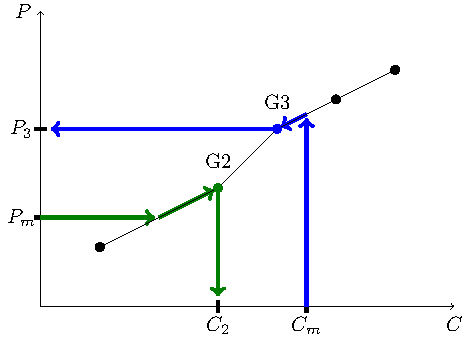
\includegraphics[width=0.7\linewidth]{images/performance-complexity-schema/performance-complexity-schema.pdf}
	\caption{Achieving the target operating point by means of the performance-complexity trade-off. In case of minimal required performance (green arrows), we find the graph $G_2$, where the model achieves at least performance $P_m$. In case of maximal available resources (blue arrows), we select the model achieving performance $P_3$. Original figure from \cite{prochazka_scalable_2022}.}
	\label{fig:performance-complexity-schema}
\end{figure}

This procedure describes a basic way of choosing a \textbf{working point} that is optimal for the particular use-case. The choice of the working point, suitable performance metric and complexity metric are subjective and depend on the particular use-case, downstream task and the environment in which the model is to be deployed. In this work, the transductive node classification accuracy on a testing dataset is chosen as the performance metric. For the complexity metric, the number of nodes in the graph was chosen as it constitutes a good proxy for real-world algorithmic complexity, as shown in \cite{chiang_cluster-gcn_2019}.

\section{A HARP-based method for performance-complexity balancing}

This method builds on the HARP method introduced in \cite{chen_harp_2018} for pretraining methods such as node2vec on coarsened graphs. The sequence \( G_0, G_1, G_2, \dots, G_L \) is generated in HARP consecutively. In an overview, the HARP algorithm first ahead-of-time consecutively coarsens the graph. The method itself can then be executed by repeating the following steps on the graphs from the coarsest to the finest (i.e., from \( G_L \) to \( G_0 \)):
\begin{enumerate}
	\item \textbf{Training on an intermediary graph}. The graph embedding model is trained on \( G_i \), producing its embedding \( \Phi_{G_i} \).
	\item \textbf{Embedding prolongation}. The embedding \( \Phi_{G_i} \) is \textit{prolonged} into \( \Phi_{G_{i - 1}} \) by copying embeddings of merged nodes. \( \Phi_{G_{i - 1}} \) is then used as the starting point for training on \( G_{i - 1} \).
\end{enumerate}

While the prolongation used by HARP is sufficient when used as a means of pre-training, the approach is far too crude when studying the relationship between graph complexity and the quality of graph embedding. In order to overcome this limitation, we present the adaptive prolongation approach. This algorithm works with the pre-coarsened graphs produced by HARP, however, the embedding is learned in a different manner. There are \( K \) prolongation steps (where generally \( K \neq L \)) and each of them uses all graphs \( G_L, \dots, G_0 \). The prolongation steps are driven by local properties of the graph with relation to the downstream task, allowing for different levels of granularity in different parts of the graph. Let us denote \( \Psi_K, \dots, \Psi_0 \) the resulting embedding sequence. The algorithm starts with the coarsest graph \( G_L \), trains a graph model to compute its embedding \( \Psi_K \) and gradually refines it until reaching the embedding \( \Psi_0 \). These prolongation steps are interlaid with continued training of the graph model, as in standard HARP\@. A description of a single prolongation step from \( \Psi_{i + 1} \) to \( \Psi_i \) is schematically outlined in Figure~\ref{fig:adaptive-prolongation} and described in detail in \cite{dedic_balancing_2023}.

\begin{figure}
	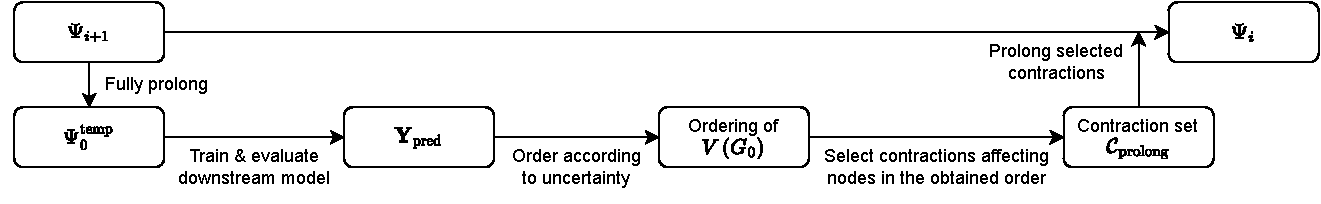
\includegraphics[width=\linewidth]{images/adaptive-prolongation/adaptive-prolongation.pdf}
	\caption{A schematic explanation of the adaptive prolongation algorithm for obtaining the embedding \( \Psi_{i} \) from \( \Psi_{i + 1} \). Original figure from \cite{dedic_balancing_2024}.}
	\label{fig:adaptive-prolongation}
\end{figure}

In \cite{dedic_balancing_2024}, we experimentally evaluated this method on 10 of the most common datasets used for graph machine learning, giving us the performance-complexity curves shown in Figure~\ref{fig:adaptive-coarsening}. The results were further verified using both null hypothesis significance testing as well as the Bayesian Wilcoxon signed-rank test (see \cite{benavoli_bayesian_2014}) with the headline result that at 60\% complexity, the models have over a 99\% probability of being within 10 percentage points of performance on the full graph and at 80\% complexity, they have over 99\% probability of being withing 5 percentage points of performance.

\begin{figure}
	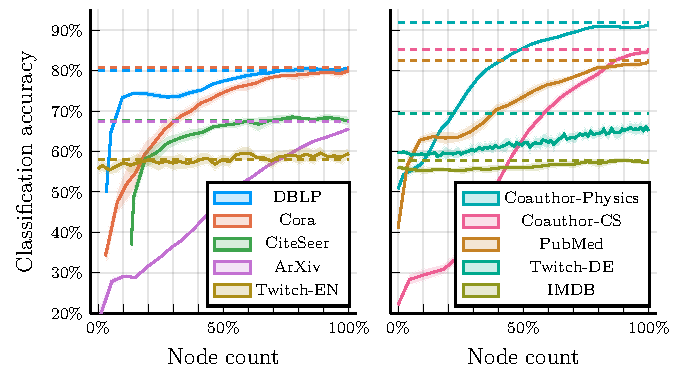
\includegraphics[width=0.8\linewidth]{images/adaptive-coarsening/adaptive-coarsening.pdf}
	\caption{Downstream classifier test-set accuracies at different steps of adaptive prolongation. Dashed line shows the baseline node2vec model accuracy. The node count is taken relative to the total node count in each dataset. The results are averaged over multiple runs, with the solid line representing the mean and the shaded area denoting one standard deviation. Original figure from \cite{dedic_balancing_2024}.}
	\label{fig:adaptive-coarsening}
\end{figure}












\begin{itemize}
	\item Graph coarsening for efficient GNNs -- direct edge collapsing (\cite{prochazka_scalable_2022})
	\item Graph properties and their role in classification and its performance (\cite{prochazka_which_2023})
	\item Maybe something more recent with explainability?
\end{itemize}
